\section{Text Classification in Legal Judgments}

% Explain the overall idea of the experiments

% How did we get to this setup?

% É possível usar TM techniques para classificar corretamente as sentenças?


This sections presents the results from the classification experiments involving JEC documents.

\subsection{Pipeline for classification}

% Create Figure for pipeline
In the experiments with classification of the JEC legal cases, we applied the open-source software Orange 3. Such tool aims at offering a variety of ML and TM techniques to the user in a simple way, without the need of any programming language. The classification in Orange3 followed the pipeline from Figure~\ref{fig:cap4_pipeline_superv_ml}.


% Adaptar aqui: veio da parte de baixo.
Foram realizados dois experimentos, sendo um com o texto integral da sentença e outro com a retirada da parte dispositiva, isto é, do texto que representa o resultado processual. Essa estratégia foi adotada para possibilitar uma comparação do desempenho das técnicas onde a classe é indicada no corpus textual e onde a classe não é indicada no corpus textual.


% TODO: add N-gram as step in the pipeline.
\begin{figure}[htb]
    \centering
    \caption{Pipeline for supervised Learning in Texts}
    \label{fig:cap4_pipeline_superv_ml}
    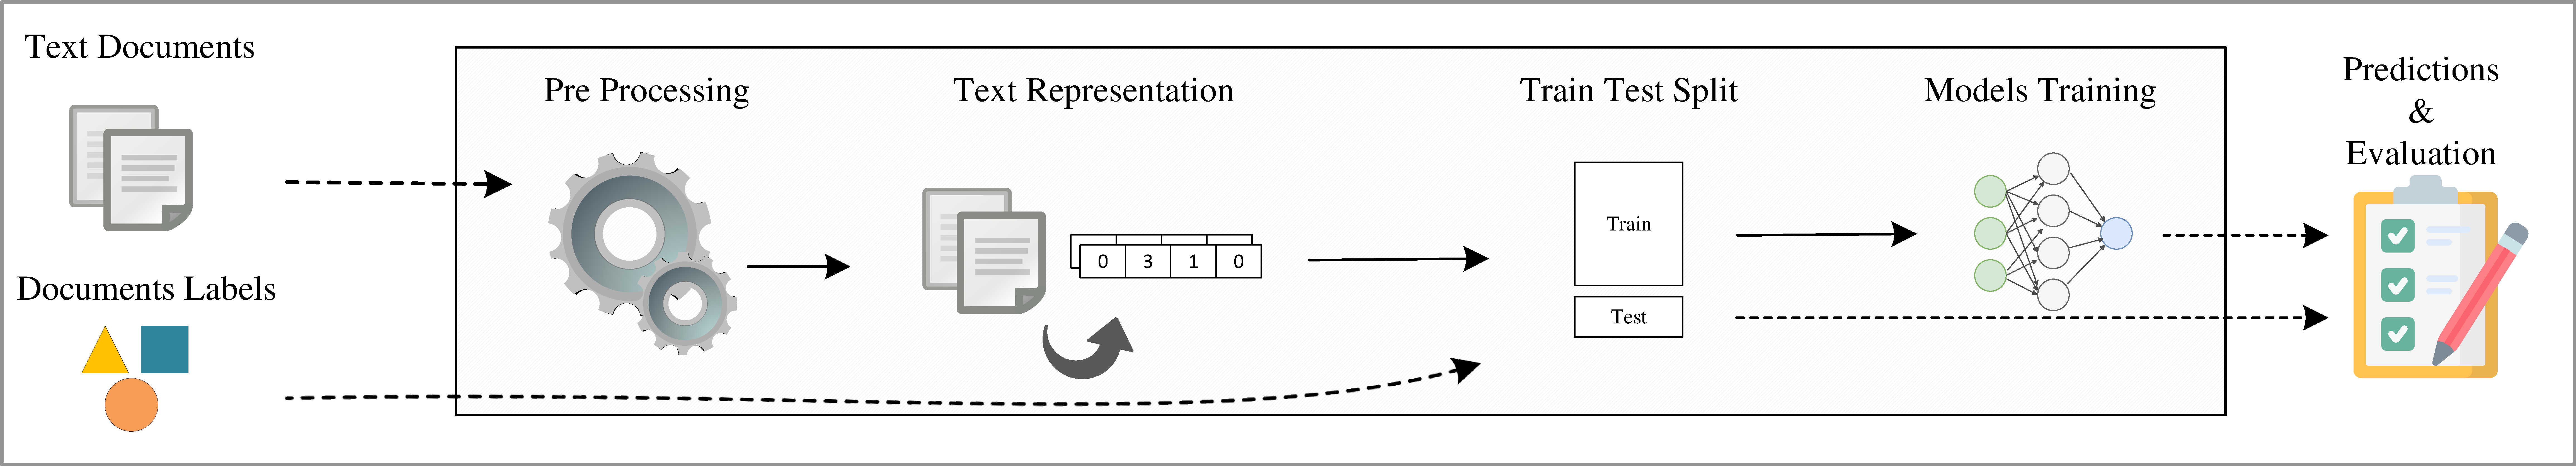
\includegraphics[width=\textwidth]{images/chapters/cap4_simple_pipeline.pdf}

\end{figure}

The pipeline from Figure \ref{fig:cap4_pipeline_superv_ml} represents a simple way to apply ML techniques to texts. It receives two types of input: the texts from legal documents, in a plan text format, and its labels, that is, the cases' results.

In the case of study, the first step in the pipeline is the data pre-processing, consisting on a set of techniques to prepare the data to serve as input to an algorithm (GARCÍA; LUENGO; HERRERA, 2015). Considering the available techniques for pre-processing data described in Chapter 2 and literature in Appendix \ref{ap:rsl_ml_law}, in this work, the following techniques were applied:

\begin{itemize}
    \item \textbf{Tranformation:} the conversion to lower case to standardize the spelling of words.
    \item \textbf{Tokenization:} the application of regular expression ($\setminus w+$) to detect the pieces of texts, while removing spaces, symbols, and punctuation.
    \item \textbf{Stemming:} To reduce the variability of similar words, we applied Porter Stemmer (CITE), a simple and efficient stemming algorithm to the Portuguese language. However, it may make errors such as contracting the word \textit{morais} to \textit{morai}, instead of \textit{moral} (Portuguese words for singular and plural of \textit{moral}, respectively).
    \item \textbf{Filtering:} Removing stopwords, such as prepositions and articles to keep only the meaningful words. Orange makes available a list of stopwords in the Portuguese language that include words like \textit{de} (of/from), \textit{para} (for), \textit{alguns} (some).
\end{itemize}



The next step in the pipeline relates to the extraction of N-Grams which detects sequences of two or more words that appear together consistently in the text. Examples of such sequences include \textit{text mining}, \textit{air transport} and others. In this research, the limit of the length of N-grams was two. Bigger numbers of N-grams would lead to unreasonably large textual representations.


%%%%%%%%%%%%%%%%%%%%%%%%%%%%%%%%%%%%%%%%%%%%%%%%%%%%%%%

Nas etapas de stemização e filtro foi necessário a especificação de um dicionário da língua portuguesa.
Essas etapas de pré-processamento têm como resultado a geração de uma bag of words (bolsa de palavras), na qual cada documento é representado como um vetor de palavras que ocorrem no documento. Nela é efetuada a contagem dos termos e o cálculo da frequência em que cada termo aparece no documento (MATSUBARA; MARTINS; MONARD, 2003).

After N-Grams Extraction, the numerical representations of the documents are created using the algorithm Bag of Words (BOW). In this work, we used the Term Frequency to set the values of the BOW model. 


Having the representation of the texts, the next step consists on dividing the dataset in two subsets: train and test sets. As described in Chapter \ref{cap:ml_text} (CHECK), among the methods to do so, there is the cross validation, which splits the dataset in $k$ folds, where $k-1$ are used for training and $1$ for testing the models. In $k$ steps, cross-validation alternates folds in such a way that each of them is used to train and test the ML models. In this research, $k$ was set to 10, that is, 90\% of the dataset used for training and 10\% for testing the models.

The next step consists on training the models to predict the result of the cases from JEC according to the possible outcomes, as described in Section \ref{sec:dataset_construction}. 

In this research, we tested the following techniques: k-Nearest Neighbors (kNN), Support Vector Machines (SVM), Random Forest (RF), feed-forward Neural Networks (NN), Naïve Bayes (NB) and Logistic Regression (LR). Table \ref{tab:hyperparam_classification} presents the hyper-parameters applied to each technique, based on the values suggested by Orange 3.


% Incluir Tabela para descrever os parâmetros dos modelos.
\begin{table}[htb]
\centering
\caption{Hyperparameters for classification techniques}
\label{tab:hyperparam_classification}
\begin{tabular}{@{}cl@{}}
\toprule
\textbf{Technique} & \multicolumn{1}{c}{\textbf{Hyper-parameters}}                                                                                                                                \\ \midrule
kNN                & \begin{tabular}[c]{@{}l@{}}Number of Neighbors: 4;\\ Distance Metric: Euclidean;\\ Weight: Uniform;\end{tabular}                                                       \\ \hdashline
LR                 & \begin{tabular}[c]{@{}l@{}}Regularization type: Ridge (L2);\\ C (strength): 1\end{tabular}                                                                             \\ \hdashline
NB                 & --                                                                                                                                                                     \\ \hdashline
NN                 & \begin{tabular}[c]{@{}l@{}}Hidden Layers: 2\\ Neurons in each layer: 100, 50;\\ Activation Function: tanh;\\Solver: Stochastic Gradient descent (SGD)\end{tabular}                                                      \\ \hdashline
RF                 & \begin{tabular}[c]{@{}l@{}}Number of Trees: 10;\\ Minimum subset size: 5\end{tabular}                                                                                  \\ \hdashline
SVM                & \begin{tabular}[c]{@{}l@{}}C (cost): 1.0;\\ $\epsilon$ (Regression loss): 0.1;\\ Kernel: Radial Basis Function (RBF);\\ Iteration Limit: 100\end{tabular} \\ \bottomrule
\end{tabular}
\end{table}


After the ten steps of the cross validation, there is the evaluation step, which takes as input the trained models and the test set, and evaluate how well the models perform on classifying unseen legal cases. To estimate the performance, we use the Accuracy, detailed in \ref{cap:ml_text}.

The following section presents the results for the two experiments using the pipeline from Figure \ref{fig:cap4_pipeline_superv_ml}.

\subsection{Results and Discussion for classification experiments}


The results obtained after applying to the pipeline from Figure \ref{fig:cap4_pipeline_superv_ml} are presented in the following paragraphs.

% Continuar daqui
Table \ref{tab:cap4_class_with_result} shows the accuracy obtained for each algorithm on each label using the full cases' text.





% Please add the following required packages to your document preamble:
% \usepackage{booktabs}
% \caption{Acurácia da classificação com o dispositivo das sentenças}
\begin{table}[htb]
\centering
\caption{Classification accuracy for the dataset with cases' result}
\label{tab:cap4_class_with_result}
\begin{tabular}{crrrrr}
\hline
\textbf{Technique} & \multicolumn{1}{c}{\textbf{\begin{tabular}[c]{@{}c@{}}Well\\ Founded\end{tabular}}} & \multicolumn{1}{c}{\textbf{\begin{tabular}[c]{@{}c@{}}Partly\\ founded\end{tabular}}} & \multicolumn{1}{c}{\textbf{\begin{tabular}[c]{@{}c@{}}Not\\ founded\end{tabular}}} & \multicolumn{1}{c}{\textbf{\begin{tabular}[c]{@{}c@{}}Dismissed\\ without\\ prejudice\end{tabular}}} & \multicolumn{1}{c}{\textbf{\begin{tabular}[c]{@{}c@{}}Micro\\ Accuracy\end{tabular}}} \\ \hline
kNN                & 75,9\%                                                                              & 71,9\%                                                                                & 93,5\%                                                                             & 95,7\%                                                                                               & 75,8\%                                                                                \\\hdashline
SVM                & 34,3\%                                                                              & 45,5\%                                                                                & 89,6\%                                                                             & 98,5\%                                                                                               & 47,3\%                                                                                \\\hdashline
RF                 & 82,6\%                                                                              & 82,6\%                                                                                & 96,1\%                                                                             & 97,9\%                                                                                               & 84,2\%                                                                                \\\hdashline
NN                 & 85,9\%                                                                              & 84,9\%                                                                                & 97,5\%                                                                             & 97,9\%                                                                                               & 86,7\%                                                                                \\\hdashline
NB                 & 75,2\%                                                                              & 47,3\%                                                                                & 91,4\%                                                                             & 19,6\%                                                                                               & 60,3\%                                                                                \\\hdashline
LR                 & 87,1\%                                                                              & 86,2\%                                                                                & 97,6\%                                                                             & 97,9\%                                                                                               & 87,8\%                                                                                \\ \hline
\end{tabular}

Source: Adapted from \textcite{Sabo2019}
\end{table}

On the one hand, there is the highest performance of LR, followed by NN, for the \emph{Well Founded}, \emph{Partially Founded} and \emph{Not founded} labels. On the other hand, there is a significantly lower performance from the SVM for the \emph{Well Founded} and \emph{Partially Founded} labels, while in NB for the \emph{Partially Founded} label. However, for the \emph{Dismissed without prejudice} label, whose sample is smaller, the SVM achieved the highest performance, while the Naïve Bayes significantly achieved the lowest. The accuracy achieved by each classifier can be better compared in Figure 2. 

\begin{figure}[htb]
    \centering
    \caption{Classification accuracy for the dataset with cases' result}
    \label{fig:cap4_class_with_result}
    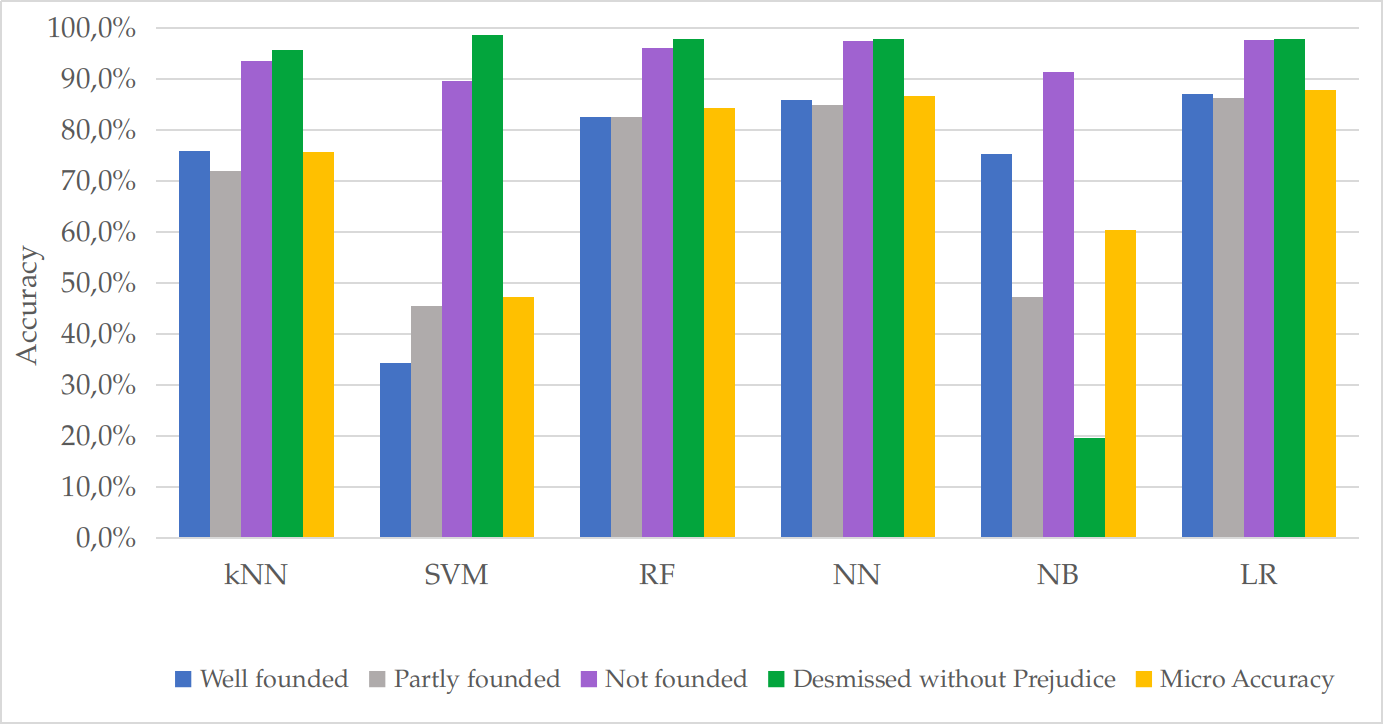
\includegraphics[width=\textwidth]{images/chapters/cap4_classification_with_result.png}
    
    Source: Adapted from \textcite{Sabo2019}
\end{figure}

Table \ref{tab:cap4_class_without_result} contains the accuracy achieved by each algorithm in each of the four labels using the text of the cases without result of the process. 


\begin{table}[htb]
\centering
\caption{Classification accuracy for the dataset without cases' result}
\label{tab:cap4_class_without_result}
\begin{tabular}{@{}crrrrr@{}}
\toprule
\textbf{Technique} & \multicolumn{1}{c}{\textbf{\begin{tabular}[c]{@{}c@{}}Well\\ founded\end{tabular}}} & \multicolumn{1}{c}{\textbf{\begin{tabular}[c]{@{}c@{}}Partly\\ founded\end{tabular}}} & \multicolumn{1}{c}{\textbf{\begin{tabular}[c]{@{}c@{}}Not\\ founded\end{tabular}}} & \multicolumn{1}{c}{\textbf{\begin{tabular}[c]{@{}c@{}}Dismissed\\ without\\ prejudice\end{tabular}}} & \multicolumn{1}{c}{\textbf{\begin{tabular}[c]{@{}c@{}}Micro\\ Accuracy\end{tabular}}} \\ \midrule
kNN                & 75,2\%                                                                              & 72,1\%                                                                                & 90,9\%                                                                             & 93,2\%                                                                                               & 75,4\%                                                                                  \\\hdashline
LR                 & 80,7\%                                                                              & 79,2\%                                                                                & 94,9\%                                                                             & 97,9\%                                                                                               & 81,6\%                                                                                  \\\hdashline
NB                 & 74,3\%                                                                              & 46,5\%                                                                                & 90,2\%                                                                             & 18,1\%                                                                                               & 59,5\%                                                                                  \\\hdashline
NN                 & 81,0\%                                                                              & 79,0\%                                                                                & 95,1\%                                                                             & 97,9\%                                                                                               & 81,6\%                                                                                  \\\hdashline
RF                 & 82,2\%                                                                              & 79,9\%                                                                                & 92,7\%                                                                             & 97,9\%                                                                                               & 82,2\%                                                                                  \\\hdashline
SVM                & 33,4\%                                                                              & 45,0\%                                                                                & 89,6\%                                                                             & 98,5\%                                                                                               & 46,7\%                                                                                  \\ \bottomrule
\end{tabular}

Source: Adapted from \textcite{Sabo2019}
\end{table}


On the one hand, there is the highest performance of RF, followed by NN and LR, for the \textit{Well founded}, \emph{Partially founded} and \emph{Not founded} classes. On the other hand, there is a significantly lower performance of the SVM for the \textit{Well founded} and \emph{Partially founded} labels, and NB for the  \emph{Partially founded} labels. However, for the \emph{Dismissed without prejudice} label, whose sample is smaller, again the SVM achieved the highest performance, while the NB obtained a significantly lower result. The accuracy achieved by each classifier can be better compared in Figure 3. 


\begin{figure}[htb]
    \centering
    \caption{Classification Accuracy for the dataset without cases' results}
    \label{fig:cap4_class_without_result}
    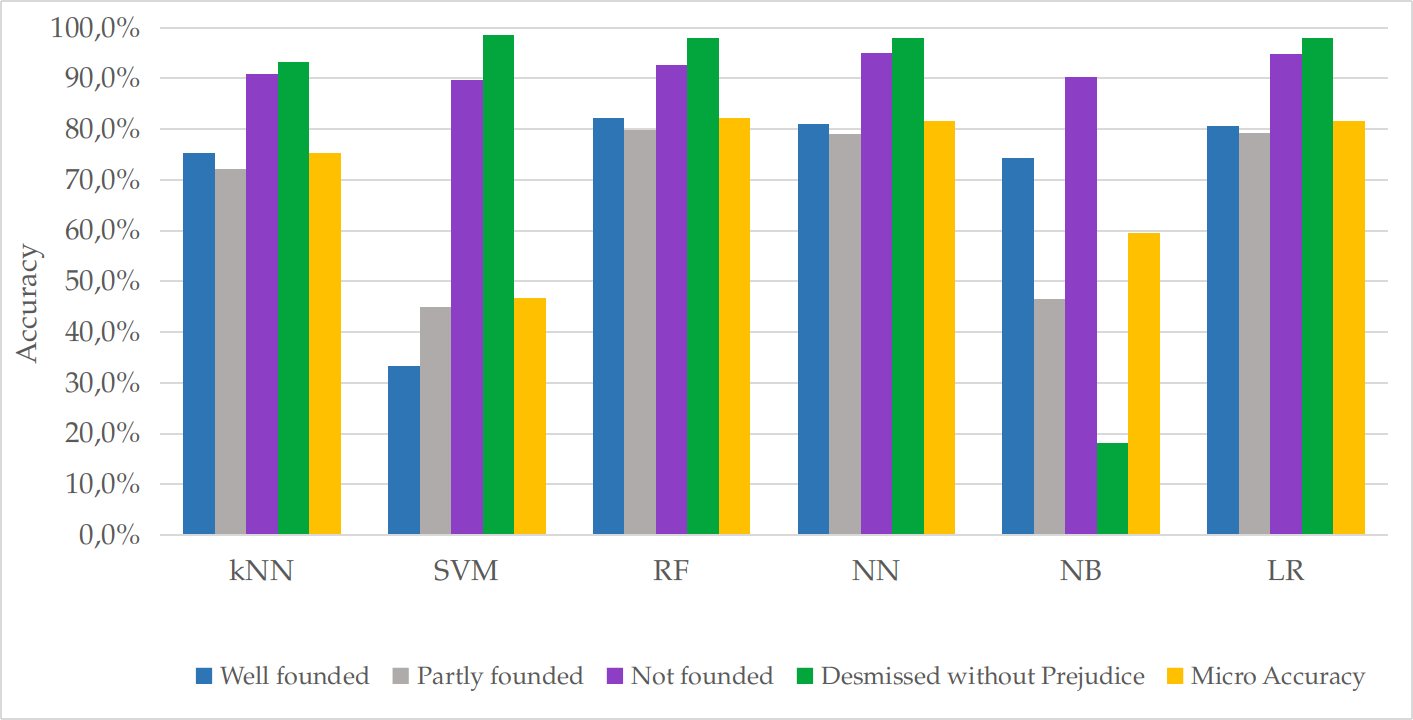
\includegraphics[width=\textwidth]{images/chapters/cap4_classification_without_result.png}
    
    Source: Adapted from \textcite{Sabo2019}
\end{figure}


Table 3 shows the difference in accuracy between the experiments, indicating an average of the accuracy obtained by each classifier in the four labels. 

% Table aqui

In general, it is inferred from the averages that the accuracy in the experiment with the removal of the cases' result (part of the text indicating the label to which it belongs) suffered a minimal reduction, which demonstrates that the classifiers only maintained their performance with the text in which the facts narrated by the parties to the process are reported and the legal grounds applicable to the case. This becomes a prerequisite for carrying out experiments with texts from legal proceedings in which there is still no sentence, that is, in which the judge has not yet decided the result. 

It is also observed that the greatest difference was obtained with the LR for the \textit{partly founded} label, whose sample is larger, while the difference obtained by the kNN for the same class was negative, which means that this classifier performed better on the text of cases without the result. 

\subsection{Conclusions from the section}

The experiments from this section dealt with initial experiments carried out in the sentences of the JEC/UFSC, indicating only four possible classes to which the texts belong. In general, it was possible to obtain an overview of how the several ML techniques behave in the face of legal texts (specific on Consumer Law and failure in air transport service), evaluating which classification models reached higher and lower accuracy.

%As future works, the aim is to improve the text representation of the bag of words for a more robust representation, such as Word Embeddings, capable of numerically associating contexts and semantics to words. In addition, we intend to build a new structure for sentence prediction, composed of cascading classifiers, using attributes extracted from texts through clustering. Thus, it is possible to make intermediate classifications that will serve as a basis for a final classification. 